\newpage
%\section{Introduction}
\chapter{Introduction}
\label{sec:introduction}
\section{Motivation}

This master thesis is part of the NTNU SmallSat \cite{SmallSat_project_description} project. The projects mission is to use hyperspectral imaging to observe ocean color in the ocean and the coast of Norway. The payload of the satellite will be a 1/3 U push-broom type hyperspectral imager (HSI), dedicated to take images of a $30x30 km^2$. In regular Red Green Blue(RGB) imaging each of the image pixels is made up of three frequency components that represent the intensities in red, green and blue frequencies respectively. Such a component is referred to as a band. In hyperspectral imaging, a pixel will typically consists of hundreds to thousands of bands, providing more information than regular images. This information can be used for a lot of different purposes. It can for example be used to detect different materials in an area, by using spectral signatures of materials as identifiers. This is shown in Figure \ref{fig:HSI_concept}.\\

\begin{figure}[H]
\centering
   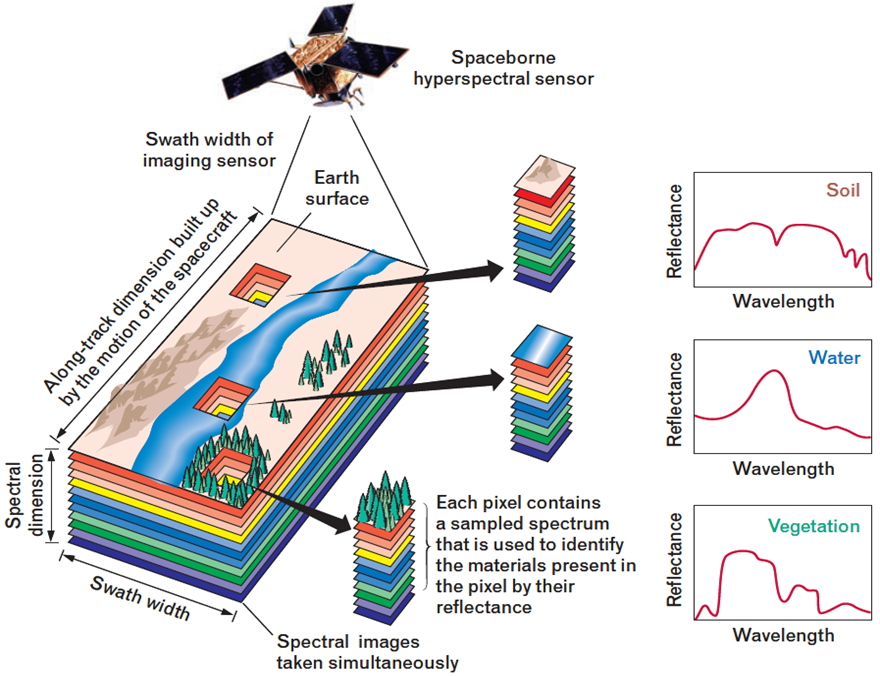
\includegraphics[scale=0.3]{images/Imaging-Spectroscopy-Concept.png}
  \caption{ Functional concept of HSI.\cite{HSI_concept} } 
  \label{fig:HSI_concept}
\end{figure}


NTNU SmallSat aims to use this information to detect algae blooms, phytoplankton and possibly other irregularities or \textit{anomalies} in the ocean. Detection of algae blooms is particularly interesting for the salmon farms located along the coast of Norway, as such blooms can be toxic, even deadly, for the salmon. Algaes were most likely the cause of death for 38 000 salmons in southern Troms in September of 2017 \cite{laksedeath}. An image of such a bloom can be seen in Figure \ref{fig:algae_bloom_troms}.  %With the increasing rise in sea temperatures and the issues faced with global warming this is an even 
% HSI  = hyperspectral imager or imaging?
\\

\begin{figure}[H]
\centering
   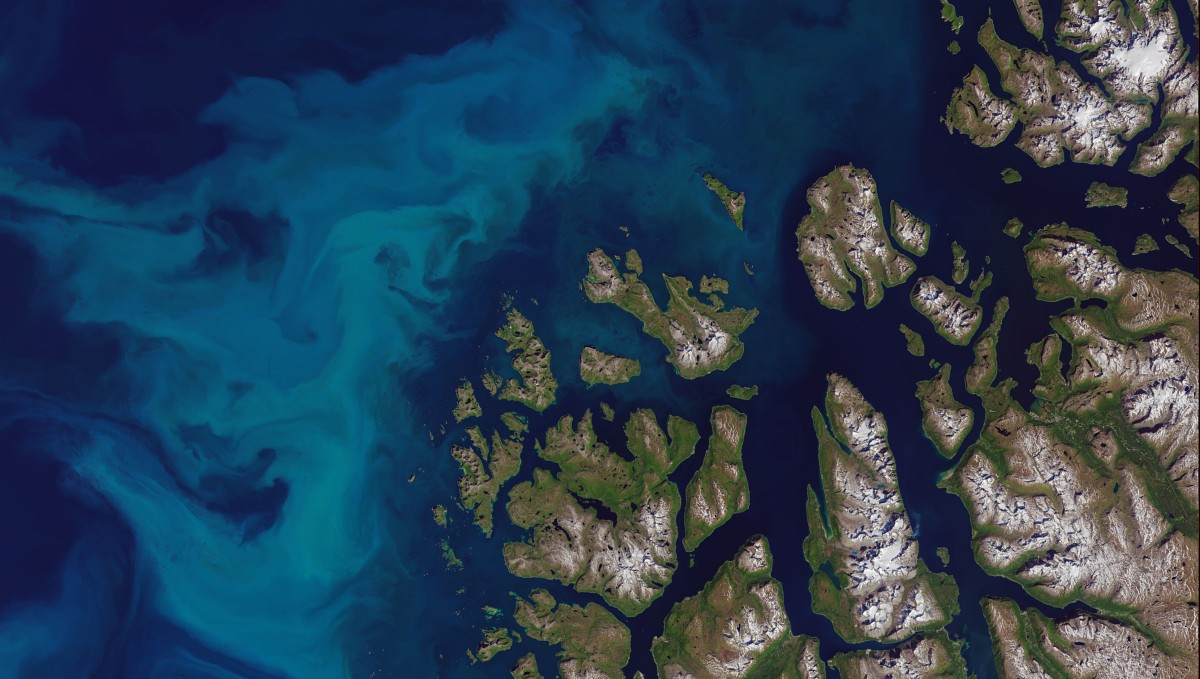
\includegraphics[scale=0.3]{images/algaes/algaes_northern_troms.jpg}
  \caption{ Image of an algae bloom along the coast of Troms in Norway \cite{laksedeath}. Foto by NASA EARTH OBSERVATORY. } 
  \label{fig:algae_bloom_troms}
\end{figure}
\\

Algaes will have spectral signature that is different to the background, which will be ocean water or land. It may therefore be considered an \textit{anomaly}. An anomaly in the context of HSI is a pixel vector that have significant spectral differences from its surrounding background pixels \cite{yang2015dual}.  
\\
As hyperspectral images contain a lot of data, and the transmission time is short(*Something something transmission while over area*, reaction time...)
 
 





\newpage
\subsection{Project report overview}
The following chapters in this project report delve into the design of a miniature camera on the Disruptive Technology sensor platform. Different image sensors will be considered, with respect to design parameters such as size, battery lifetime, energy, power dissipation and area of application. Three different system alternatives with different system partitioning are analyzed and evaluated. One system is proposed for implementation.\\  

Chapter \ref{sec:theory} is the Theory section. 


Chapter \ref{sec:methodology} is the Methodology section. 


Chapter \ref{sec:results} is the Results section. Results from estimations of energy consumption, battery-capacity consumption and power dissipation are presented here based on methodology presented in chapter \ref{sec:methodology}. Also, experimental results from doing image processing on pictures taken with the NanEye2D image sensor are presented here. 
\\

Chapter \ref{sec:Discussion} is the Discussion section. The results of the energy and power estimations for the three system alternatives are discussed here. A comparison of the different alternatives is made based on metrics such as number of frames possible to capture, process and transmit, area of application and compression rate possible. 
\\

Chapter \ref{sec:conclusion} is the Conclusion section. The most important results are presented here. The proposed system of the miniature camera is presented as well. Future work that can be done is mentioned, listed in bullet-points. 
\\




